\documentclass[11pt]{article}
\usepackage[a4paper,margin=27mm]{geometry}
\usepackage{amsmath,amssymb,amsthm,mathtools,booktabs,graphicx,microtype,xcolor}
\usepackage[hidelinks]{hyperref}
\usepackage{listings}
\usepackage{fancyhdr}
\pagestyle{fancy}\fancyhf{}\lhead{Coefficient budgets for Burgers singularities}\rhead{Shivam Gupta}\cfoot{\thepage}
\setlength{\headheight}{14pt}
\newtheorem{theorem}{Theorem}\newtheorem{proposition}[theorem]{Proposition}\newtheorem{corollary}[theorem]{Corollary}\newtheorem{lemma}[theorem]{Lemma}
\newcommand{\C}{\mathbb C}\newcommand{\R}{\mathbb R}\newcommand{\Z}{\mathbb Z}\newcommand{\e}{\mathrm e}\newcommand{\ii}{\mathrm i}\newcommand{\dd}{\,\mathrm d}
\DeclareMathOperator{\conv}{conv}\DeclareMathOperator{\Rea}{Re}\DeclareMathOperator{\Ima}{Im}
\title{Sharp Coefficient Budgets for Certified\newline Singularity Counts in Periodic Burgers Flow}
\author{Shivam Gupta\\Independent Researcher\\\texttt{shivam1720406@gmail.com}}
\date{17 October 2026}
\begin{document}\maketitle
\begin{abstract}
Complex singularities of viscous Burgers solutions are routinely estimated through analytic continuation, but a computed pole pattern does not specify how much uncertainty in the input preserves its contour count. We study additive $\ell^1$ uncertainty in the Fourier coefficients of the initial Cole--Hopf potential. For positive heat time, we characterize the exact distance to a boundary zero in both unrestricted complex and real-data-preserving perturbation classes. The complex value set is a disk with an explicitly computable, finite critical frequency. The real value set is the convex hull of a sequence of Fourier ellipses; its gauge gives the exact distance, and at most two mode blocks attain it. A constructive example requires two blocks and uses a budget of one where the best single pair requires $1.2352\ldots$. An Arb-based implementation combines these formulas with a proved infinite-series tail bound and validated winding numbers. All 16 contours of a designed Burgers benchmark yield certified counts and two-sided budget enclosures. At heat time $1/2$ and contour half-height one, real-data-preserving uncertainty admits a guaranteed budget over 64\% larger than the complex class. These results provide an explicit error-budget interface between spectral data and complex singularity diagnostics, with a separate positivity condition for smooth real Burgers initial data.
\end{abstract}
\noindent\textbf{Keywords:} complex singularities; Burgers equation; Cole--Hopf transformation; coefficient uncertainty; validated numerics; structured value sets.

\section{Introduction}
Complex singularities encode useful information about solutions of nonlinear partial differential equations, including the distance over which an analytic continuation remains regular. For viscous Burgers flow, the Cole--Hopf transformation reduces singularity detection to finding zeros of an entire heat potential. This makes the equation a particularly transparent setting in which to distinguish two questions: where does a nominal computation place singularities, and which topological statements survive an explicitly specified error in its inputs?

We investigate the second question for periodic heat potentials with absolutely summable initial Fourier coefficients. The uncertainty is attached to those coefficients before heat evolution. This placement matters: heat smoothing suppresses high frequencies on the real line, while continuation to imaginary height $y$ amplifies one sign of the Fourier modes. Their competition selects a finite damaging frequency. Requiring the uncertain initial potential to remain real on the real line couples opposite frequencies and changes the attainable perturbations from a disk to a convex hull of ellipses.

Our contribution is a complete specialization of structured zero-exclusion geometry to this infinite Fourier heat family, together with a reproducible validated implementation. The central result identifies exact boundary-zero distances for both perturbation classes. It also gives sparse extremizers, a finite support-function evaluation with a proved mode cutoff, and a positivity cap needed when the potential represents a smooth real Burgers initial condition. The experiments then quantify the difference between the two classes without estimating a pole trajectory or fitting a rational model.

The scope is deliberately precise. A budget below the distance guarantees an unchanged zero count on a fixed contour. Attaining the distance creates a boundary zero; it need not produce a different count in every direction beyond that threshold. The count is of heat zeros with their algebraic multiplicities. A zero of order $m$ gives a simple pole of the Burgers logarithmic derivative with residue $-2\nu m$, so zero multiplicity must not be confused with the order of that pole.

\section{Related work and research positioning}
Weideman's Fourier-based continuation method computes complex singularity dynamics from spectral solutions \cite{weideman}. VandenHeuvel et al. combine exact formulas, asymptotics, and AAA approximation to study Burgers singularities \cite{vandenheuvel}. Their analysis of pole motion provides important context; the present work instead asks how a specified coefficient uncertainty changes a contour-count guarantee.

Zeros of heat solutions and complex Burgers singularities are classically connected through Cole--Hopf; Pol\'a\v cik and \v Sver\'ak study the development and isolation of complex-valued singularities \cite{polacik}. Our use of the logarithmic derivative is part of this established framework.

The general principles behind the robustness calculation are also established. Polyak and Halpern treat infinite-dimensional $\ell^1$ uncertainty using value sets and zero exclusion \cite{polyak}. Michiels et al. give structured pseudospectral formulas and discuss their relationship with stability radii for analytic matrix functions \cite{michiels}. We do not claim a new general zero-exclusion theorem. The specific object here is the bilateral Fourier heat family, including its conjugate-symmetric perturbations, its finite critical-mode calculations, and its use as an error budget for Burgers diagnostics.

Rigorous contour-based root counting predates this work: Schaefer develops an interval argument-principle method for analytic zeros \cite{henrici}, and Johnson and Tucker give guaranteed zero enclosures in rectangles \cite{johnson}. The winding-number implementation below is a compact application of that tradition, with an explicit infinite Fourier remainder. Arb supplies the underlying ball arithmetic \cite{johansson}. The literature search did not establish a precedent combining this particular real-symmetric Fourier uncertainty geometry, sparse witnesses, and a validated Burgers contour-budget study. That is the contribution claimed here; the search does not prove the absence of every equivalent formulation.

\section{Heat potentials, contours, and uncertainty}
Let $\nu>0$, $t>0$, and $\tau=\nu t$. For $c\in\ell^1(\Z;\C)$ define
\begin{equation}\label{eq:heat}
 \Phi_c(z,\tau)=\sum_{k\in\Z} c_k\e^{-\tau k^2}\e^{\ii kz}.
\end{equation}
On each bounded complex strip the series, with any fixed number of spatial derivatives, converges normally: the Gaussian factor dominates every exponential in $|k|$. Thus $\Phi_c$ is entire. Where $\Phi_c$ is nonzero,
\begin{equation}\label{eq:burgers}
 u(z,t)=-2\nu\,\frac{\partial_z\Phi_c(z,\nu t)}{\Phi_c(z,\nu t)}
\end{equation}
solves $u_t+uu_z=\nu u_{zz}$. If $\Phi_c=(z-z_0)^m g$ with $g(z_0)\ne0$, then $u=-2\nu m/(z-z_0)-2\nu g'/g$.

Let $\Gamma$ be the positively oriented boundary of a bounded Jordan domain and assume $\Phi_c\ne0$ on $\Gamma$. Write
\begin{equation}
 Z_\Gamma(c)=\frac{1}{2\pi\ii}\int_\Gamma\frac{\partial_z\Phi_c}{\Phi_c}\dd z.
\end{equation}
This integer counts interior heat zeros with multiplicities. We consider perturbations $d$ with $\|d\|_1=\sum_k|d_k|$. The unrestricted class is $d\in\ell^1(\Z;\C)$. In the real class, both the nominal and perturbed initial potentials satisfy $c_{-k}=\overline{c_k}$ and $d_{-k}=\overline{d_k}$, with real constant coefficient. Then
\begin{equation}\label{eq:realnorm}
 \|d\|_1=|d_0|+2\sum_{k\ge1}|d_k|.
\end{equation}
The norm is a global coefficient budget, rather than an independent error bar for every coefficient or a bound on sampled velocity errors.

Define the boundary-zero distances
\begin{equation}\label{eq:distance}
 \rho_X(c,\Gamma)=\inf\{\|d\|_1:\Phi_{c+d}(z,\tau)=0
 \text{ for some }z\in\Gamma,\ d\in X\},\qquad X\in\{\C,\R\}.
\end{equation}
The notation $\R$ denotes conjugate symmetry, not real coefficients for every positive Fourier mode. At fixed positive $\tau$ and compact $\Gamma$, evaluation is a continuous map from $\ell^1$ into continuous boundary functions.

\section{Exact complex budgets and the critical frequency}
\begin{theorem}\label{thm:complex}
For $y\in\R$ set
\begin{equation}\label{eq:A}
 A_\tau(y)=\max_{k\in\Z}\e^{-\tau k^2-ky}
 =\exp\!\left(\max_{j\ge0}\{j|y|-\tau j^2\}\right).
\end{equation}
The value set $\{\Phi_d(x+\ii y,\tau):\|d\|_1\le\epsilon\}$ is the closed disk of radius $\epsilon A_\tau(y)$. Consequently
\begin{equation}\label{eq:complexradius}
 \rho_\C(c,\Gamma)=\min_{z\in\Gamma}\frac{|\Phi_c(z,\tau)|}{A_\tau(\Ima z)}.
\end{equation}
The pointwise distance is attained by a perturbation supported on a single integer mode. A maximizing $j$ is an integer nearest to $|y|/(2\tau)$, with both adjacent integers admissible at a tie.
\end{theorem}
\begin{proof}
Absolute summation gives $|\Phi_d(z)|\le A_\tau(y)\|d\|_1$. The exponent in \eqref{eq:A} tends to $-\infty$ as $|k|\to\infty$, so its maximum is attained. If $k_*$ maximizes it, any $w$ in the disk is realized by $d_{k_*}=w\e^{\tau k_*^2-\ii k_*z}$ and all other coefficients zero. The least norm producing $w=-\Phi_c(z)$ is therefore $|\Phi_c(z)|/A_\tau(y)$. This expression is continuous on the compact boundary, proving the minimum formula. Completing the square yields the nearest-integer rule.
\end{proof}
\begin{corollary}\label{cor:complexcount}
If $\|d\|_1<\rho_\C$, then $Z_\Gamma(c+d)=Z_\Gamma(c)$. At norm $\rho_\C$ a boundary zero is attainable.
\end{corollary}
\begin{proof}
The strict inequality implies $|\Phi_d|<|\Phi_c|$ everywhere on the boundary, so Rouch\'e's theorem applies. Attainment follows from Theorem~\ref{thm:complex} at a minimizing boundary point.
\end{proof}
A useful interpretation is frequency selection rather than unrestricted high-frequency instability. At fixed $\tau>0$ and $y$, modes beyond the Gaussian maximum become less damaging. As $\tau\downarrow0$ for nonzero $y$, the maximizer escapes to infinity; no fixed finite cutoff is uniform in that limit.

\begin{figure}[t]\centering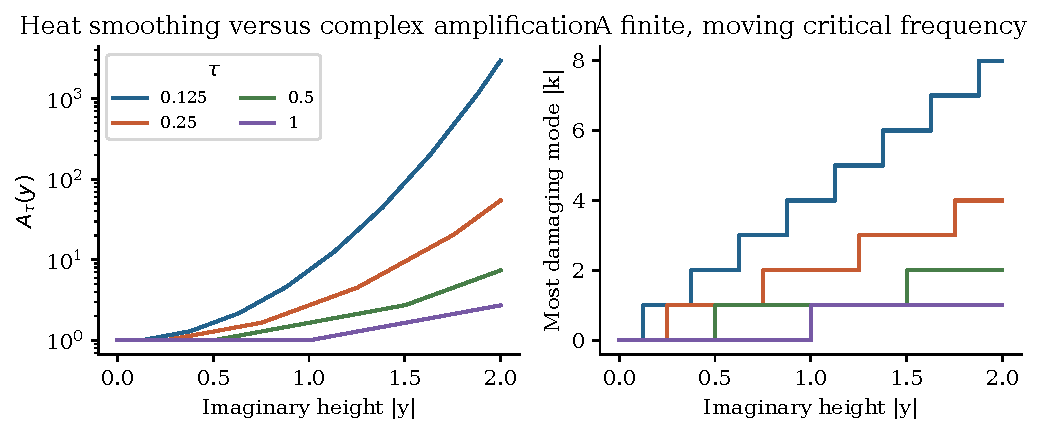
\includegraphics[width=\linewidth]{../figures/amplification.pdf}
\caption{The exact complex evaluation norm and its critical frequency. Curves use \eqref{eq:A}; colors correspond to heat times. Heat smoothing makes the infinite-mode uncertainty norm finite at every positive time.}\label{fig:amp}\end{figure}

\section{Real data: Fourier ellipses and sparse extremizers}
Put $y=|\Ima z|$. For $k\ge1$ let
\begin{equation}\label{eq:ellipse}
 E_k(y)=\left\{a_k(y)\cos\alpha+\ii b_k(y)\sin\alpha:
 \alpha\in[0,2\pi]\right\}_{\rm filled},\quad
 \begin{cases}a_k=\e^{-\tau k^2}\cosh(ky),\\b_k=\e^{-\tau k^2}\sinh(ky),\end{cases}
\end{equation}
and let $E_0=[-1,1]$. The filled-ellipse convention includes the interior. Let $K_\tau(y)=\conv\bigcup_{k\ge0}E_k(y)$.

\begin{theorem}\label{thm:real}
For conjugate-symmetric $d$, the unit-budget value set at $x+\ii y$ is exactly $K_\tau(|y|)$, independently of $x$. Its support function is
\begin{equation}\label{eq:h}
 h_\tau(\theta,y)=\max_{k\ge0}\e^{-\tau k^2}
 \sqrt{\cosh^2(ky)\cos^2\theta+\sinh^2(ky)\sin^2\theta}.
\end{equation}
For $y>0$, its gauge is
\begin{equation}\label{eq:gauge}
 g_{\tau,y}(w)=\max_{\theta\in[0,2\pi]}
 \frac{\Rea(\e^{-\ii\theta}w)}{h_\tau(\theta,y)}.
\end{equation}
For a real nominal potential,
\begin{equation}\label{eq:realradius}
 \rho_\R(c,\Gamma)=\min_{z\in\Gamma}g_{\tau,|\Ima z|}(-\Phi_c(z,\tau)),
\end{equation}
where $g_{\tau,0}(w)=|w|$ for real $w$. Every pointwise minimum for $y>0$ is attained using at most two mode blocks: each block is either the constant mode or one conjugate pair. Norms below $\rho_\R$ preserve $Z_\Gamma$.
\end{theorem}
\begin{proof}
Write $d_k=(r/2)\e^{\ii\alpha}$. The $k,-k$ contribution is
\begin{equation}
 \e^{-\tau k^2}\bigl(d_k\e^{\ii kz}+\overline{d_k}\e^{-\ii kz}\bigr)
 =r\e^{-\tau k^2}\{\cos(\alpha+kx)\cosh(ky)-\ii\sin(\alpha+kx)\sinh(ky)\}.
\end{equation}
Its cost is $r$, so it traces the boundary of $rE_k$. Allowing smaller amplitude fills the ellipse. Distributing the total norm between blocks gives precisely the convex hull. Conversely, every finite convex combination is realized by such coefficients with total cost at most one. The ellipses shrink uniformly to the origin as $k\to\infty$; their union is compact after including the origin, already in $E_0$. Its convex hull in $\R^2$ is compact, so the attainable set is closed and no closure correction is needed.

The support of a filled axis-aligned ellipse is the square root in \eqref{eq:h}; the support of a convex hull is the maximum of the supports. Since $E_1$ has positive semiaxes for $y>0$, $K_\tau(y)$ contains a neighborhood of zero. The supporting-halfspace description of a closed convex body then gives \eqref{eq:gauge}.

For $w\ne0$, the normalized target $p=w/g_{\tau,y}(w)$ lies on a supporting line of $K_\tau(y)$. Every point on this exposed face is a convex combination of at most two endpoints of that face. Each endpoint is an extreme point of the convex hull of the compact union, hence belongs to one of the ellipses. This supplies a two-block representation with total cost $g_{\tau,y}(w)$. For $w=0$ take $d=0$.

At $y=0$ all attainable values are real, and the constant mode attains the interval $[-1,1]$; the nominal boundary value is also real. To justify the minimum on $\Gamma$, take a minimizing sequence of boundary points and perturbations with uniformly bounded norms. The coefficient balls are weak-* compact in $\ell^1=(c_0)^*$, and the evaluation sequences in \eqref{eq:heat} belong to $c_0$ and vary continuously there on compact strips. After passing to subsequences, their evaluations converge to that of a limiting conjugate-symmetric perturbation at a limiting boundary point. Lower semicontinuity of the norm proves attainment and hence the minimum in \eqref{eq:realradius}.

If $\|d\|_1<\rho_\R$, the path $c+sd$, $0\le s\le1$, cannot encounter a boundary zero by the definition of $\rho_\R$. Its winding number is consequently constant.\end{proof}

On the real axis the target must remain real. For an arbitrary imaginary target there is a genuine degeneracy, as the following result shows.

\begin{proposition}[No uniform real--complex equivalence]\label{prop:gap}
For fixed $\tau>0$,
\begin{equation}
 g_{\tau,y}(\ii)=\frac{1}{\max_{k\ge1}\e^{-\tau k^2}\sinh(ky)}
 \sim \frac{1}{y\max_{k\ge1}k\e^{-\tau k^2}},\qquad y\downarrow0,
\end{equation}
whereas the unrestricted complex distance to the same unit imaginary target tends to one. Thus there is no uniform constant bounding real-symmetric pointwise distances by complex distances for arbitrary targets.
\end{proposition}
\begin{proof}
The greatest imaginary coordinate in $K_\tau(y)$ is $\max b_k(y)$ and is attained on the imaginary axis of an ellipse. The first formula follows. Dominated convergence, using $\sinh(ky)/y\le k\e^{ky}$ for bounded positive $y$, gives uniform convergence of the relevant weighted sequences to $k\e^{-\tau k^2}$. Finally, $A_\tau(y)\to1$.
\end{proof}
This operator statement is not a claim of divergent gains for the particular positive Burgers family below.

\subsection{Two blocks can be necessary}
At $\tau=y=1$, let $a=\e^{-1}\cosh1$, $b=\e^{-1}\sinh1$ and
\begin{equation}\label{eq:two}
 \tan\theta_*={\sqrt{1-a^2}\over b},\qquad
 p_0=(1,0),\quad p_1=(a^2,b^2\tan\theta_*),\quad w_*={p_0+p_1\over2}.
\end{equation}
For $k\ge1$, both $\e^{-k^2}\cosh k$ and $\e^{-k^2}\sinh k$ strictly decrease: their logarithmic derivatives are $-2k+\tanh k$ and $-2k+\coth k$, respectively, both negative for $k\ge1$. Hence every $E_k$, $k\ge2$, lies inside $E_1$. The line with normal $(\cos\theta_*,\sin\theta_*)$ supports both $E_0$ at $p_0$ and $E_1$ at $p_1$. The target $w_*$ therefore has exact gauge one and is attained by spending half the budget on each block. It lies outside $E_1$, while its imaginary part precludes a constant-only representation. The least single-pair cost is
\begin{equation}
 \sqrt{(\Rea w_*/a)^2+(\Ima w_*/b)^2}=1.2352341853\ldots.
\end{equation}
The two-block cost is 19.04\% below that single-pair cost; equivalently the single-pair restriction requires 23.52\% more budget. This is a value-set example, not a claim that $w_*$ is generated by the positive benchmark's boundary minimum.

\begin{figure}[t]\centering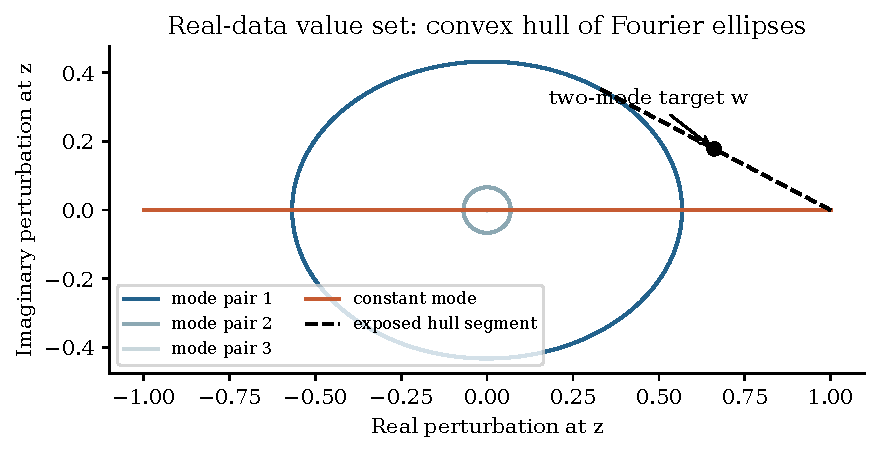
\includegraphics[width=.95\linewidth]{../figures/geometry.pdf}
\caption{A constant mode and a conjugate pair can be jointly necessary. At $\tau=y=1$, the marked target lies on a hull segment outside every single ellipse. Its cost is one; a single pair costs $1.235234\ldots$. Smaller ellipses are shown for context.}\label{fig:geom}\end{figure}

\section{Smooth real initial data and normalization}
Real symmetry alone does not ensure that the initial Cole--Hopf potential is positive. If $\phi_0(x)=\sum c_k\e^{\ii kx}$ is real and $\phi_0(x)\ge m_0>0$, then every real-symmetric perturbation of norm below $m_0$ remains positive, because $|\sum d_k\e^{\ii kx}|\le\|d\|_1$. The real heat equation preserves positivity, yielding a smooth real Burgers solution for all real $t>0$.

For the benchmark $\phi_0(x)=\e^{a\cos x}$, $m_0=\e^{-a}$. This positivity radius is exact: the constant perturbation $d_0=-\e^{-a}$ makes the initial potential vanish at $x=\pi$. Thus the guarantee that simultaneously preserves initial positivity and the chosen contour count is
\begin{equation}\label{eq:cap}
 \|d\|_1<\min\{\e^{-a},\rho_\R(c,\Gamma)\}.
\end{equation}
The computed $\rho_\R$ itself is the boundary-zero distance in the entire real-symmetric coefficient class; it is not asserted to be the exact boundary-zero distance after additionally imposing positivity. Equation~\eqref{eq:cap} avoids this distinction being hidden in a numerical table.

Multiplying the potential by a positive constant leaves $u$ unchanged but scales absolute coefficient budgets. We fix the normalization $\phi_0=\e^{a\cos x}$ throughout. Its initial coefficient norm is $\e^a$, so a scale-invariant relative budget is $\rho_X/\e^a$ when the nominal and uncertainty are scaled together.

\section{Validated numerical method}
\subsection{Infinite support reduced to a checked finite maximum}
For \eqref{eq:A}, completing the square already identifies the finite candidates. For the real support function at $y>0$,
\begin{equation}
 h_1(\theta,y)\ge\e^{-\tau}\sinh y,\qquad
 h_k(\theta,y)\le\e^{-\tau k^2+ky}.
\end{equation}
Choose $K>y/\tau$ such that
\begin{equation}\label{eq:cutoff}
 \e^{-\tau(K+1)^2+(K+1)y}<\e^{-\tau}\sinh y.
\end{equation}
The right-hand envelope decreases for all subsequent integers. No $k>K$ can maximize the support function. The code proposes $K$ in floating point, then verifies \eqref{eq:cutoff} using Arb comparisons and increases it until the test succeeds. This is an exact cutoff for the uncertainty set, distinct from the truncation of the nominal potential.

\subsection{Nominal Fourier tail}
The standard Bessel generating function gives \cite{dlmf}
\begin{equation}\label{eq:bessel}
 \Phi(z,\tau)=I_0(a)+2\sum_{k\ge1}I_k(a)\e^{-\tau k^2}\cos(kz),\qquad
 u(x,0)=2\nu a\sin x.
\end{equation}
Let $n=N+1$ and $Y\ge|\Ima z|$. From the power series for $I_k$ and $(k+j)!\ge k!(k+1)^j$,
\begin{equation}
 I_k(a)\le\frac{(a/2)^k}{k!}\exp\!\left(\frac{a^2}{4(k+1)}\right).
\end{equation}
Since $|\cos(kz)|\le\cosh(kY)\le\e^{kY}$, successive majorant terms for $k\ge n$ have ratio at most
\begin{equation}
 q=\frac{a}{2(n+1)}\exp\{Y-\tau(2n+1)\}.
\end{equation}
When $q<1$, the omitted tail obeys
\begin{equation}\label{eq:tail}
 |\Phi-\Phi_N|\le B_N(Y):=
 \frac{2(a/2)^n}{n!(1-q)}
 \exp\!\left\{\frac{a^2}{4(n+1)}-\tau n^2+nY\right\}.
\end{equation}
All quantities, including the Bessel coefficients, are evaluated with outward ball bounds. The code adds $[-B_N,B_N]+\ii[-B_N,B_N]$, a rectangle containing the tail disk.

For a boundary segment contained in a complex rectangle $Q$ with center $m$ and $r^2=\sup_{z\in Q}|z-m|^2$, the finite part is evaluated using
\begin{equation}\label{eq:taylor}
 \Phi_N(z)\in\Phi_N(m)+\Phi_N'(m)(Q-m)+D(0,M_2r^2/2),\qquad
 M_2=2\sum_{k=1}^N k^2I_k(a)\e^{-\tau k^2}\cosh(kY).
\end{equation}
Taylor's integral remainder along the straight line from $m$ to $z$ proves this enclosure. Adding \eqref{eq:tail} accounts for every omitted mode. Near-point evaluations use the direct series. Both paths are inclusions; a heuristic switch affects enclosure width, not validity.

\subsection{Winding numbers and two-sided distances}
The contour starts with four oriented rectangle edges. An edge is bisected until its enclosed image is a convex rectangle excluding the origin. Such an image lies in an open half-plane through the origin, so the true phase change along that edge is the principal argument of the ratio of endpoint values. Summing interval principal arguments and dividing by $2\pi$ encloses the winding number. A count is returned only when this ball lies strictly within $(n-1/4,n+1/4)$ for one integer $n$. A depth cap or an ambiguous sum returns \texttt{unresolved}.

For a segment $Q$, the complex lower bound is
\begin{equation}
 L_\C(Q)=\frac{\inf|\Phi(Q)|}{\sup A_\tau(|\Ima Q|)}.
\end{equation}
A midpoint $z_m$ gives the upper bound $|\Phi(z_m)|/A_\tau(|\Ima z_m|)$. For real uncertainty, any chosen direction $\theta$ gives a rigorous dual lower bound
\begin{equation}\label{eq:dualbound}
 L_\R(Q)\ge
 \frac{\inf_{z\in Q}\Rea[-\e^{-\ii\theta}\Phi(z)]}
 {h_\tau(\theta,\max_{z\in Q}|\Ima z|)}
\end{equation}
when the numerator is positive. The denominator is valid because every ellipse expands monotonically with $|y|$. The implementation takes the maximum of this and the complex lower bound. A floating-point angular optimization proposes $\theta$; the entire resulting inequality is recomputed with Arb. Optimizer success is not an acceptance condition.

Real upper bounds are constructive. A single pair $k$ realizes any complex target $w$ at $y>0$ for cost
\begin{equation}\label{eq:single}
 C_k(w)=\sqrt{(\Rea w/a_k)^2+(\Ima w/b_k)^2}.
\end{equation}
The code also evaluates support points of candidate ellipses. If interval solution of $w=\lambda p_k+\mu p_l$ verifies $\lambda,\mu\ge0$, then $\lambda+\mu$ is a feasible cost. Inverting the corresponding two-by-two matrix with outward bounds supplies a rigorous upper bound. Searching only finitely many pairs can miss an optimal representation, but cannot invalidate an upper bound.

A branch-and-bound loop splits the boundary segment with the smallest lower bound. With $L$ the smallest retained lower bound and $U$ the best feasible upper bound, the primary stopping rule is $L\ge0.98U$. The reported enclosure is for the global minimum over the whole boundary, not a minimum over the sampled points. The implementation has finite resource caps and is not claimed to terminate for every possible input.

\section{Computational study}
\subsection{Protocol and checks}
The designed benchmark fixes $a=2$, $N=40$, and 160-bit ball precision. It uses $\tau\in\{1/8,1/4,1/2,1\}$ and $Y\in\{1/4,1/2,1,2\}$ on the positively oriented rectangle
\begin{equation}
 \Gamma_Y=\partial\{z:0\le\Rea z\le2\pi,\ -Y\le\Ima z\le Y\}.
\end{equation}
Vertical edges are included in both the count and the robustness budget. Thus the count is for this cut rectangle. A perturbation can move a zero across the cut without changing the total count on a periodic cylinder; our distance can consequently be conservative for a cylinder-only question. Every benchmark boundary is certified zero-free.

The protocol is stored as JSON with all limits. It is a recorded computational protocol, not a public preregistration. The raw results preserve ball endpoints, segment counts, evaluations, and runtime. The environment was Python 3.12.14 and Python-FLINT 0.9.0 on macOS arm64. Wall times are descriptive; no implementation-speed advantage is claimed.

Independent analytic fixtures test $1+b\e^{-\tau m^2}\cos(mz)$ for $b=1/2$, $m\in\{1,2,3\}$ and two heat times. Their zeros satisfy $\Rea z=(2j+1)\pi/m$ and
$|\Ima z|=m^{-1}\operatorname{arcosh}(\e^{\tau m^2}/b)$. Twelve inner/outer contour counts match these formulas. A boundary-zero fixture is required to return \texttt{unresolved}. Additional checks cover the norm formula, tail enclosures, primal--dual costs, invalid inputs, and the real--complex budget gap. Eight unit-test methods pass.

For three benchmark contours, eight seeded perturbations in each class are generated with support $|k|\le4$ and budget $0.45$ times the certified lower bound. All 48 perturbed winding counts equal their nominal counts. These are implementation checks on sampled perturbations; the proof supplies the guarantee over the entire norm ball, including modes beyond four. Nine additional runs vary $N\in\{24,40,56\}$ and precision in $\{96,160,224\}$ bits for the $(\tau,Y)=(1/2,1)$ case. All certify count two and converged real-radius enclosures.

\begin{figure}[t]\centering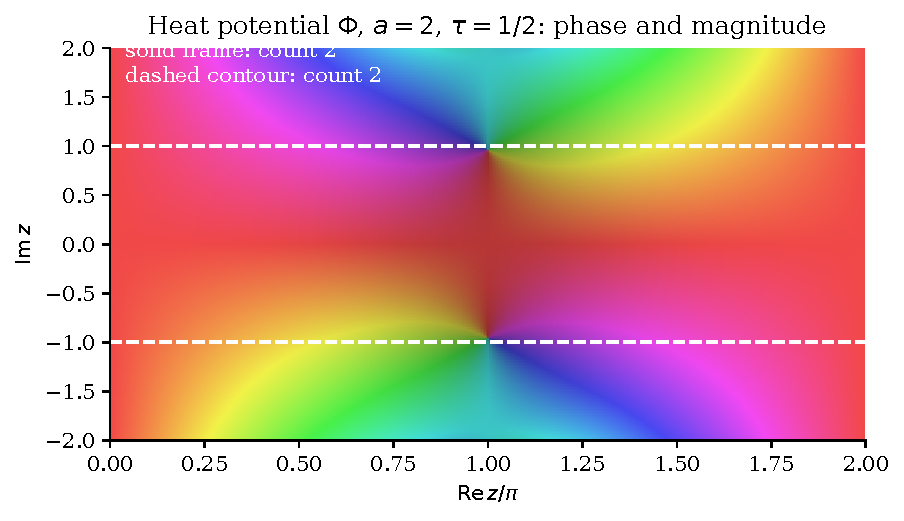
\includegraphics[width=.95\linewidth]{../figures/landscape.pdf}
\caption{Phase-and-magnitude illustration of the heat potential at $a=2$, $\tau=1/2$. The outer frame and dashed inner contour both have certified heat-zero count two. The image uses ordinary floating point for visualization; the stated counts use interval computation with the infinite tail included.}\label{fig:land}\end{figure}

\subsection{Results}
\begin{table}[t]\centering\small
\caption{Certified heat-zero counts and enclosures for boundary-zero budgets. Intervals are rounded outward from the stored ball bounds. $\rho_\R$ refers to all real-symmetric potential perturbations; smooth positive initial data additionally require \eqref{eq:cap}.}\label{tab:results}
\begin{tabular}{rrrrr}\toprule
$\tau$ & $Y$ & $Z_{\Gamma_Y}$ & $\rho_\C$ enclosure & $\rho_\R$ enclosure\\\midrule
0.125 & 0.25 & 0 & [0.1448, 0.1475] & [0.1652, 0.1686] \\
0.125 & 0.5 & 0 & [0.07451, 0.07593] & [0.124, 0.1258] \\
0.125 & 1 & 0 & [0.002477, 0.002506] & [0.004928, 0.005011] \\
0.125 & 2 & 4 & [3.244e-06, 3.311e-06] & [6.489e-06, 6.621e-06] \\
0.25 & 0.25 & 0 & [0.2384, 0.2406] & [0.24, 0.2443] \\
0.25 & 0.5 & 0 & [0.1294, 0.1319] & [0.1689, 0.1719] \\
0.25 & 1 & 2 & [0.0145, 0.0147] & [0.02847, 0.02886] \\
0.25 & 2 & 4 & [0.002481, 0.002524] & [0.004979, 0.005047] \\
0.5 & 0.25 & 0 & [0.4879, 0.4937] & [0.4933, 0.5032] \\
0.5 & 0.5 & 0 & [0.3785, 0.3806] & [0.3804, 0.3848] \\
0.5 & 1 & 2 & [0.02587, 0.02605] & [0.04289, 0.04375] \\
0.5 & 2 & 2 & [0.1051, 0.1071] & [0.2104, 0.214] \\
1 & 0.25 & 0 & [1.088, 1.101] & [1.1, 1.118] \\
1 & 0.5 & 0 & [0.9818, 0.9988] & [0.998, 1.015] \\
1 & 1 & 0 & [0.5569, 0.5681] & [0.5679, 0.5751] \\
1 & 2 & 2 & [0.5287, 0.5316] & [1.027, 1.044] \\\\\bottomrule
\end{tabular}\end{table}
All 16 nominal contours yield certified counts; all 32 budget calculations satisfy the stopping criterion on their unrounded endpoints. The counts range from zero to four. Table~\ref{tab:results} reports every planned configuration, including the least robust case. At $(\tau,Y)=(1/8,2)$ the real budget is only about $6.5\times10^{-6}$, despite a visually resolvable singularity pattern. This is a quantified conditioning limitation, not a failed computation or an assertion of physical instability.

At $(\tau,Y)=(1/2,1)$, the real lower bound $0.04289$ exceeds the complex upper bound $0.02605$ by more than 64\%. Thus the separation holds for the entire certified intervals. The real guarantee is also below $\e^{-2}\approx0.1353$, so it is compatible with the smooth-real-data condition without clipping. Relative to the nominal coefficient norm $\e^2$, these budgets are of order $0.58\%$ and $0.35\%$, respectively.

At $(\tau,Y)=(1/8,1)$, the conservative ratio of the real lower to complex upper bound exceeds $1.96$. At $(1/2,2)$ it also exceeds $1.96$, but the raw real boundary-zero radius exceeds the initial positivity cap, so the admissible smooth-real Burgers budget is smaller than the tabulated potential radius. Near the real axis several configurations show little separation, consistent with the constant mode dominating both value sets.

The budgets are not monotone in contour height, as Figure~\ref{fig:budgets} shows. Moving a boundary toward a nominal zero decreases its distance, while moving it beyond a zero can increase the margin even though the enclosed count has changed. A count alone therefore does not summarize the robustness of a singularity diagnostic. The two-sided budget supplies information that the count omits.

\begin{figure}[t]\centering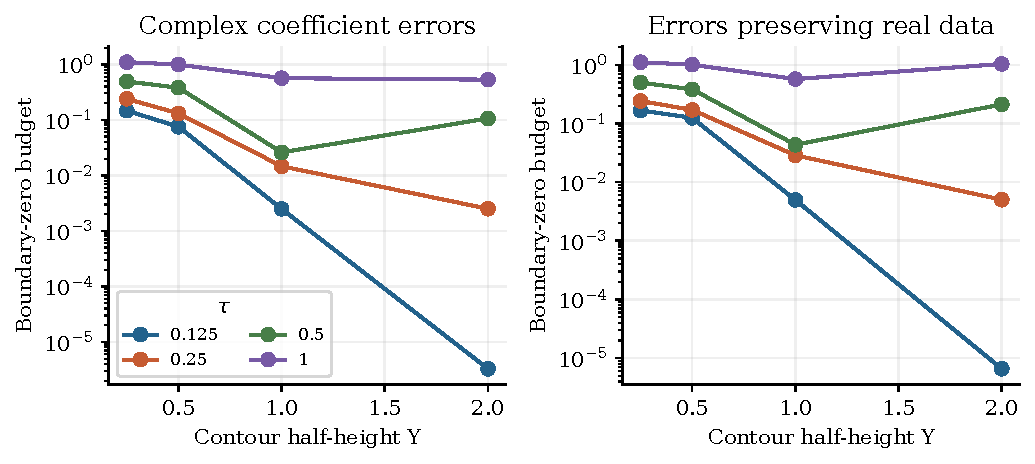
\includegraphics[width=\linewidth]{../figures/budgets.pdf}
\caption{Boundary-zero budgets over the complete designed grid. Lines join interval midpoints for readability; shading marks the validated intervals. The two panels use the same vertical scale. Each point is a global contour calculation, not a sampled-boundary minimum.}\label{fig:budgets}\end{figure}

\section{Practical use and limitations}
A spectral computation can use the result as an explicit acceptance rule: provide a normalized initial heat potential, a coefficient-norm error budget, a positive heat time, and a contour; accept a count only when the uncertainty budget is strictly below the validated lower bound. This could support regression checks for spectral PDE software, comparisons between discretizations, or a diagnostic layer around scientific surrogate models that output heat-potential coefficients. The guarantee concerns those coefficients. Converting an error estimate on velocity samples, an FFT with aliasing, or a learned representation into this norm requires additional analysis.

Existing continuation environments such as Chebfun already compute and visualize complex singularities \cite{chebfun}. A plausible software application is an uncertainty-aware verification component integrated with these workflows. The present work demonstrates the mathematics and executable component; it does not measure user demand, establish a market size, or support a patentability claim. Mature open-source numerical tools and the substantial prior art in robust zero exclusion make broad commercial-exclusivity claims inappropriate.

Several mathematical limits remain. The heat time and viscosity are treated as known; their interval uncertainty is not included in the distance theorem. The norm ball does not encode conservation constraints, fixed mean, correlated coefficient errors, or a posteriori residuals from a nonlinear PDE solver. The positivity cap is sufficient for combining the two requirements and exact for positivity alone, but does not solve the positivity-constrained boundary optimization. The fixed cut rectangle can understate robustness of a periodic-cylinder count. Multiple heat zeros are counted with multiplicity, and the code does not classify their distinct locations. All experiments concern an integrable equation and one infinite-series initial family; they do not establish a method for arbitrary nonlinear PDEs.

The numerical validation depends on the inclusion guarantees of Arb and on the correctness of the surrounding code. The study includes analytic fixtures, precision and truncation variation, and constructive primal--dual checks, but is not a formally machine-checked proof of the software. Absolute absence of equivalent prior work cannot be concluded from a finite literature search. The contribution is the explicit Fourier heat formulation and its verified use, rather than a claim to have invented contour counting, convex duality, or Cole--Hopf analysis.

\section{Conclusion}
For periodic Cole--Hopf potentials, a singularity count can be accompanied by a mathematically defined coefficient budget. Heat smoothing gives an exact disk norm for complex perturbations, while conjugate symmetry yields a convex hull of ellipses with sparse extremizers. The distinction can materially enlarge a certified budget, and a two-block example proves that restricting attention to one Fourier pair can lose optimality. Infinite-series bounds and interval contour computations turn these formulas into reproducible guarantees on a nontrivial Burgers benchmark. Extending this interface to constrained coefficient classes and certified errors produced by PDE solvers is a concrete next step.

\paragraph{Code and data availability.}
The companion repository contains the code, tests, raw results, figures, and manuscript sources:\par\smallskip
\noindent{\small\url{https://github.com/shi1720/burgers-pole-budgets}}\par\smallskip
The code is released under the MIT license. The numerical figures are generated from the included protocol and results.

\appendix
\section{Reproduction and artifact map}
The source code represents the horizontal coordinate of a contour vertex in multiples of $\pi$; the vertical coordinate is unscaled. Rational subdivisions and Arb's enclosure for $\pi$ retain the exact intended contour. A minimal calculation is:
\begin{lstlisting}[basicstyle=\ttfamily\small,breaklines=true,frame=single]
from flint import ctx
from pole_budgets import Potential, certified_count, radius_bounds
ctx.prec = 160
p = Potential(tau="0.5", a="2", N=40)
rect = ("0", "2", "-1", "1")  # x/pi endpoints; y endpoints
assert certified_count(p, rect)["count"] == 2
budget = radius_bounds(p, rect, real=True)
assert budget["converged"]
print(budget["lower"], budget["upper"])
\end{lstlisting}

\begin{table}[h]\centering\small
\begin{tabular}{ll}\toprule
Path & Role\\\midrule
\texttt{src/pole\_budgets.py} & Ball enclosures, winding count, both distances\\
\texttt{experiments/protocol.json} & Primary numerical grid and stopping limits\\
\texttt{experiments/run.py} & Execute the full primary study\\
\texttt{experiments/validate.py} & Perturbation, geometry, and sensitivity checks\\
\texttt{experiments/figures.py} & Four figures and outward-rounded table\\
\texttt{tests/test\_core.py} & Analytic fixtures and implementation checks\\
\texttt{results/grid.json} & Every primary count and budget enclosure\\
\texttt{results/validation.json} & All supplementary validation results\\
\texttt{results/environment.json} & Recorded environment and precision\\\bottomrule
\end{tabular}
\end{table}
The README supplies the commands and pinned direct dependencies. Figures use ordinary numerical arrays to visualize the computed objects; all certificate decisions are made in ball arithmetic. Increasing precision cannot repair an incorrect uncertainty model, so the input norm and real-symmetry assumptions must be established before interpreting a returned budget.

\begin{thebibliography}{12}\small\raggedright
\bibitem{weideman} J. A. C. Weideman. Computing the dynamics of complex singularities of nonlinear PDEs. \emph{SIAM Journal on Applied Dynamical Systems}, 2(2):171--186, 2003. \href{https://doi.org/10.1137/S1111111102398305}{doi:10.1137/S1111111102398305}.
\bibitem{vandenheuvel} D. J. VandenHeuvel, C. J. Lustri, J. R. King, I. W. Turner, and S. W. McCue. Burgers' equation in the complex plane. \emph{Physica D}, 448:133686, 2023. \href{https://doi.org/10.1016/j.physd.2023.133686}{doi:10.1016/j.physd.2023.133686}. Open version: \url{https://arxiv.org/abs/2208.05652}.
\bibitem{polacik} P. Pol\'a\v cik and V. \v Sver\'ak. Zeros of complex caloric functions and singularities of complex viscous Burgers equation. \emph{Journal f\"ur die reine und angewandte Mathematik}, 616:205--217, 2008. \url{https://arxiv.org/abs/math/0612506}.
\bibitem{polyak} B. T. Polyak and M. E. Halpern. Robust stability and design of linear discrete-time SISO systems under $\ell^1$ uncertainties. \emph{IEEE Transactions on Automatic Control}, 44(11):2076--2080, 1999. \href{https://doi.org/10.1109/9.802919}{doi:10.1109/9.802919}.
\bibitem{michiels} W. Michiels, K. Green, T. Wagenknecht, and S.-I. Niculescu. Pseudospectra for analytic matrix functions and application to time-delay systems. In \emph{44th IEEE Conference on Decision and Control and European Control Conference}, pp. 4336--4341, 2005. \url{https://skoge.folk.ntnu.no/prost/proceedings/cdc-ecc05/pdffiles/papers/1874.pdf}.
\bibitem{henrici} M. J. Schaefer. Precise zeros of analytic functions using interval arithmetic. \emph{Interval Computations}, 4:22--39, 1993. \url{https://interval.louisiana.edu/reliable-computing-journal/1993/interval-computations-1993-4-pp-022-039.pdf}.
\bibitem{johnson} T. Johnson and W. Tucker. Enclosing all zeros of an analytic function---a rigorous approach. \emph{Journal of Computational and Applied Mathematics}, 228(1):418--423, 2009. \href{https://doi.org/10.1016/j.cam.2008.10.014}{doi:10.1016/j.cam.2008.10.014}.
\bibitem{johansson} F. Johansson. Arb: efficient arbitrary-precision midpoint-radius interval arithmetic. \emph{IEEE Transactions on Computers}, 66(8):1281--1292, 2017. \href{https://doi.org/10.1109/TC.2017.2690633}{doi:10.1109/TC.2017.2690633}. \url{https://arxiv.org/abs/1611.02831}.
\bibitem{dlmf} F. W. J. Olver et al., editors. \emph{NIST Digital Library of Mathematical Functions}, \S\S10.25 and 10.35. \url{https://dlmf.nist.gov/10.25}; \url{https://dlmf.nist.gov/10.35}. Accessed 17 October 2026.
\bibitem{chebfun} L. N. Trefethen. Analytic continuation via rational approximation. \emph{Chebfun Example}, March 2013. \url{https://www.chebfun.org/examples/complex/AnalyticContinuation.html}.
\end{thebibliography}
\end{document}
